\section{Methodology}

\subsection{Overview}
% The main framework is shown in Figure 3. Input images are first fed into ConAug to get context-based aug- mented views, then we pass these views into the network and get character embeddings. During training, on the one hand, these embeddings are used to transcript the text through the Prediction layer; on the other hand, we project them to a fea- ture space where we conduct the contrastive loss. 

\begin{figure*}[t]
\begin{center}
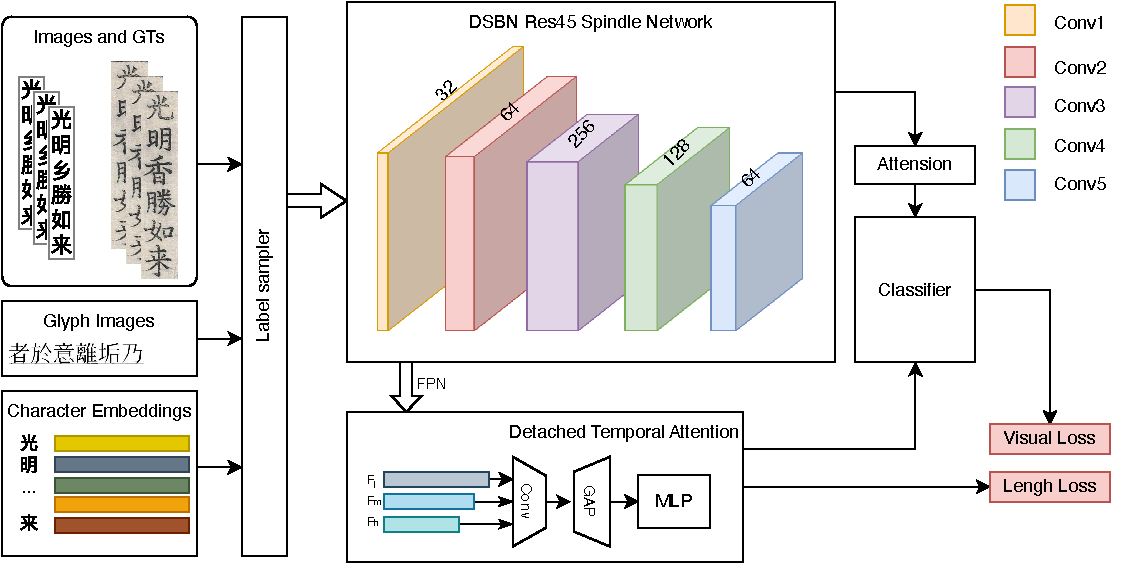
\includegraphics[width=1.0\linewidth]{figures/overall.pdf}
\end{center}
\caption{just a placeholder}
\label{fig:overall}
\end{figure*}

\subsection{Architecture}
\subsubsection{module1}
\subsubsection{module2}

\subsection{Spindle Network}





